\documentclass[a4paper]{article}

\usepackage[utf8]{inputenc}
\usepackage{tikz}
\usepackage[european, siunitx]{circuitikz}
\usepackage{floatrow}
\usepackage{mathtools}
\usepackage{cancel}
\usepackage{graphicx}
\usepackage{hyperref}

\author{Nao Pross}
\title{Sensore Termico con Arduino}

\inputencoding{utf8}

\begin{document}
	\maketitle
	%ELETTRONICA
	\section{Elettronica}
	L'intero circuito é alimentato dalla tensione di $+\SI{+5}{\volt}$ che esce dal pin dell'Arduino.
	Le misurazioni della temperatura avvengono su $V_t$ attraverso il pin di misura $Pin_{A0}$ e 
	a dipendenza del risultato viene illuminato il LED RGB. Il bottone $S_1$ permette di eseguire
	misurazioni di variazioni di temperatura più piccole.

	\begin{figure}[h]\centering \begin{circuitikz}
		%power supply
		\draw(0,0)		(0, 4)		to[voltage source,v=$+\SI{+5}{\volt}$]		(0, 0)
						(0, 4)		to[short]										(2, 4)
						%resistor
						to[R=$R_1$]												(2, 2)
						%diode
						(2, 0)		to[zD]											(2, 2)
						(2, 0)		node[above=3em, right=1em, diode]{lm335z}	(2, 0)
						to[short]													(0, 0);
		%pin A0 voltage
		\draw(2, 2)	to[short]										(3.75, 2)
						node[above=1em, led]{$Pin_{A0}$}			(3.75, 2)
						to[open, v^>=$V_t$, o-o]						(3.75, 0)
						to[short]										(5, 0);
		%button
		\draw(2, 4)	to[short]										(5, 4)
						to[push button, label=$S_1$]					(5, 2)
						to[R=330<\ohm>]								(5, 0)
						node[ground]{} 								(5, -1);
		%pin 2
		\draw(5, 2)	to[short]										(6.5, 2)
						node[above=1em, label]{$Pin_2$}				(6.5, 2)
						to[open, v^>=$V_{btn}$, o-o]					(6.5, 0)
						to[short]										(5, 0);
		%rgb led
		\draw(5, 4)	to[short]											(8, 4)
						to[leDo]											(8, 2)
						node[above=3em, right=1.5em, led]{$D_{red}$}	(8, 2)
						to[R=330<\ohm>, -o]								(8, 0)
						node[below=.5em, led]{$Pin_3$}					(8, 0);
		\draw(8, 4)	to[short]											(10, 4)
						to[leDo]											(10, 2)
						node[above=3em, right=1.5em, led]{$D_{green}$}	(10, 2)
						to[R=330<\ohm>, -o]								(10, 0)
						node[below=.5em, led]{$Pin_4$}					(10, 0);
		\draw(10, 4)
						to[short]											(12, 4)
						to[leDo]											(12, 2)
						node[above=3em, right=1.5em, led]{$D_{blue}$}	(12, 2)
						to[R=330<\ohm>, -o]								(12, 0)
						node[below=.5em, led]{$Pin_5$}					(12, 0);
	\end{circuitikz}
	\caption{Circuito Elettronico}
	\floatfoot{Nota: Il LED RGB é rappresentato con 3 diodi LED dei tre colori.}
	\end{figure}
	
	\subsection{Controllo del LED RGB}
	Il LED RGB, rappresentato nello schema come tre led $D_{red}$, $D_{green}$ e $D_{blue}$
	é combinato in tale maniera per richiedere meno potenza dalla sorgente di tensione.
	Questo sistema viene applicato spesso in elettronica ma implica che il controllo dei PIN sia
	inverso. Quindi per avere uno stato in cui $D_n$ é spento si deve generare una tensione
	di $\SI{-5}{\volt}$ dal $Pin_n$, mentre normalmente al $Pin_n$ dovrebbero esserci 
	$\SI{0}{\volt}$.\\\\
	Avere il componente collegato in tale modo implicherà delle modifiche nel software
	del circuito.
	
	%SENSORE
	\section{Sensore}
	La tensione misurata in $V_t$ é la tensione che cade sul diodo Zener LM335z, questo
	sensore é configurato per funzionare da $\SI{-40}{\celsius}$ a $\SI{+100}{\celsius}$.
	Nel datasheet é dato che a $\SI{+25}{\celsius}$ ha una tensione di $\SI{2,98}{\volt}$,
	da questo possiamo trovare attraverso una proporzione, come convertire la tensione in
	temperatura.\\
	(Nota: Nel calcolo i \SI{25}{\celsius} vengono convertiti in Kelvin)
	\begin{align*}
		\frac{V_t}{\SI{2.98}{\volt}} &= \frac{T_K}{\SI{25}{\celsius}}\\
		T_K &= \frac{\cancel{\SI{298}{\kelvin}}}{\cancel{\SI{2.98}{\volt}}}*V_t\\
		\implies T_k &= 10*V_t
	\end{align*}
	L'Arduino però legge un valore analogico come un numero intero da $0$ a $1023$, quindi per
	convertire il valore di nuovo in Volts é necessario sapere a quanto corrisponde un unità
	della misura del pin di Arduino. Dalle formule precedenti possiamo trarre una proporzione
	tra le due grandezze e quindi estrarre $V_t$.
	$$\frac{M_{A0}}{1024} = \frac{V_t}{V_{max}} \implies V_t = \frac{M_{A0} * V_{max}}{1024} ~con~0\leq M_{A0} \leq 1023$$
	$V_{max}$ può essere calcolato semplicemente attraverso la proporzione precedente, quindi
	$$V_{max} = \frac{1}{10}*T_K \implies V_{max} = \frac{\SI{373}{\kelvin}}{10} = \SI{37.3}{\kelvin}$$
	Utilizzando questo metodo creiamo una scala, e dato che la una unità in gradi Kelvin equivale a una nei
	gradi Celsius con il calcolo possiamo ottenere direttamente una temperatra in \si{\celsius}.
	$$V_t = \frac{\SI{37.3}{\kelvin}}{1024} * M_{A0}$$
	$$T_{\si{\celsius}} = 10 * V_t$$

	%SOFTWARE
	\section{Software}
	\subsection{Rappresentazione}
	Per rappresentare la temperatura ambiente con il circuito ho deciso di utilizzare il LED RGB,
	avendo la formula per convertire l'input del sensore in \si{\celsius} posso anche andare nella
	direzione opposta. Quindi la luminosità del LED sarà proporzionale alla temperatura.
	Inoltre potendo utilizzare i colori ho pensato di rappresentare in rosso le temperature 
	superiori a \SI{0}{\celsius}, in blu le temperature inferiori a \SI{0}{\celsius} e in verde la
	temperatura di esattamente \SI{0}{\celsius}.\\\\
	Purtroppo però in tale modo sarebbe difficile dimostrare il funzionamento del circuito, quindi
	ho aggiunto un bottone $S_1$ che permette di spostare la referenza. Nel momento in cui $S_1$ 
	viene premuto la temperatura letta viene impostata come referenza e utilizzata al posto di
	\SI{0}{\celsius}. Di nuovo quindi il LED sarà rosso se la temperatura é maggiore della 
	referenza, blu se inferiore e verde se uguale. In questo modo la misurazione sarà molto
	sensibile e il led cambierà colore molto frequentemente poiché in una stanza la temperatura
	ambiente non é costante ma cambia in continuazione ($\pm\SI{.06}{\celsius}$).
	
	\subsection{Codice Sorgente}
	Il codice sorgente in C++ si trova sul mio GitHub in un repository
	chiamato $2samb\_hw\_and\_sw$ nella cartella $\_00\_thermal\_sensor$ o più semplicemente
	al seguente link: \\
	\url{https://github.com/NaoPross/samb2_hw_and_sw/tree/master/_00_thermal_sensor}

	\subsection{Struttogrammi}
	
	%TODO: draw structograms with vectors
	\begin{figure}[h!]
		\centering
		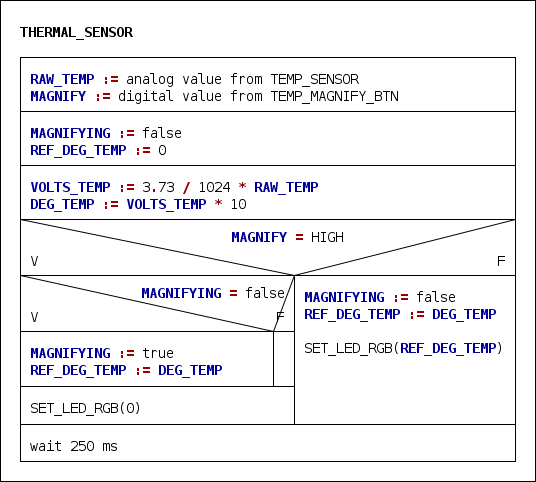
\includegraphics[width=\textwidth]{../structograms/THERMAL_SENSOR.png}
		\caption{Diagramma Nassi-Schneiderman del programma}
		\floatfoot{Nel programma é utilizzata una funzione SET\_LED\_RGB descritta nello schema successivo.}
	\end{figure}
	
	%TODO: draw structograms with vectors
	\begin{figure}[h!]
		\centering
		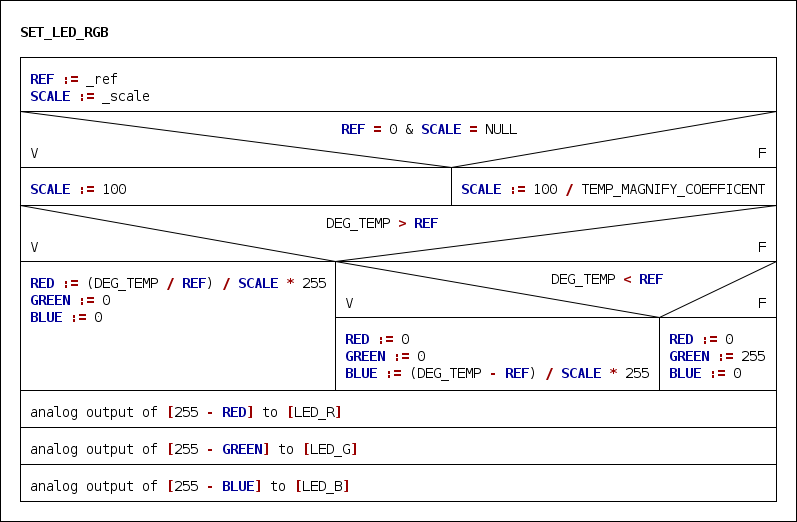
\includegraphics[width=\textwidth]{../structograms/SET_LED_RGB.png}
		\caption{Diagramma Nassi-Schneiderman della funzione SET\_LED\_RGB}
	\end{figure}
	
	
	
\end{document}
